% This is samplepaper.tex, a sample chapter demonstrating the
% LLNCS macro package for Springer Computer Science proceedings;
% Version 2.20 of 2017/10/04
%
\documentclass[runningheads]{llncs}
%
\usepackage{graphicx}
% Used for displaying a sample figure. If possible, figure files should
% be included in EPS format.
%
% If you use the hyperref package, please uncomment the following line
% to display URLs in blue roman font according to Springer's eBook style:
% \renewcommand\UrlFont{\color{blue}\rmfamily}

\usepackage{times}
\usepackage{latexsym}
\usepackage{amsmath}
\usepackage{algorithm}
\usepackage{algorithmicx}
\usepackage{amsfonts}
\usepackage{amssymb}
\usepackage{bm}
\usepackage{multirow}
\usepackage{threeparttable}
\usepackage{multicol}
\usepackage{setspace}
\usepackage{algpseudocode} 
\usepackage{soul}
\begin{document}
	%
	\title{Synthesis of Registered Multimodal
		Medical Images with Lesions}
	%
	%\titlerunning{Abbreviated paper title}
	% If the paper title is too long for the running head, you can set
	% an abbreviated paper title here
	%\inst{1}
	\author{ Yili Qu\inst{1} \and Wanqi Su\inst{1} \and Xuan Lv\inst{2} \and Chufu Deng\inst{1} 
		\and Yutong Lu\inst{1,2} \and Zhiguang Chen\inst{1} \and Nong Xiao\inst{1,2}}
	%
	\authorrunning{Y. Qu, W. Su et al.}
	% First names are abbreviated in the running head.
	% If there are more than two authors, 'et al.' is used.
	%
	\institute{Sun Yat-sen University, Guangzhou, China\\
		\email{\{quyli,suwq7,chufd3\}@mail2.sysu.edu.cn}\\\and
		National University of Defense Technology, Changsha, China\\
		\email{lvxuan14@nudt.edu.cn}
	}
	%
	\maketitle       % typeset the header of the contribution
	%
	\begin{abstract}
		The collection and annotation of medical image data have always been a challenge in many data-driven medical image processing tasks, especially for registered multimodal medical image data. This can be effectively alleviated by utilizing the image synthesis technology. However, directly-synthesized medical images generated by current methods usually have unreasonable structures or contours and uncontrollable lesions. In this paper, we proposed a new method for the synthesis of registered multimodal medical images from a random normal distribution matrix based on the Generative Adversarial Networks. Besides, the corresponding lesions can be generated efficiently based on the selected lesion labels. We perform extensive validation experiments on multiple public datasets to comprehensively verify the effectiveness of synthetic lesions and the availability of synthetic data. The results show that our synthetic data can be used as pre-trained data or enhanced data in medical image intelligent processing tasks to greatly improve the generalization ability of the model. 
		
		\keywords{Image Synthesis \and Medical Images \and Multimodal \and Lesions.}
	\end{abstract}
	%
	%
	%
	\section{Introduction}
	Intelligent medical image processing has attracted interest in the applications of deep learning (DL) technology in recent years. Medical images used for diagnosis are obtained in forms of different modalities by utilizing various imaging techniques. The common modalities include magnetic resonance imaging (MRI), computed tomography (CT), Xray, etc. Some of them have different submodalities according to different settings during imaging, e.g. MRI has submodalities of T1, T2, etc. More and more DL-based medical image studies expect large amounts of medical image data. However, the collection and annotation of medical image data remain challenging, especially for the registration of multimodal data. With the development of image synthesis technology, synthesis of high-quality medical images has become a promising method to alleviate the scarcity of medical images data.
	
	Medical images contain complex physiological structure information, and the normal method of synthesis is likely to produce unreasonable structures or contours. Moreover, it is difficult to ensure the registration when multimodal images are synthesized. Additionally, lesion information in medical images is an important basis for doctors to make diagnosis and for reasoning and diagnosis of intelligent medical image processing model. Therefore, another challenge in synthesizing medical images is to control the synthesis of lesions and generate corresponding lesion labels.
	
	Generative Adversarial Networks (GAN) have been intensively studied in medical image segmentation\cite{40kamnitsas2017unsupervised}, reconstruction\cite{61fan2018a}, synthesis \cite{41costa2017towards,4shin2018medical,43iglesias2013is,44shrivastava2017learning}, translation \cite{2zhang2018translating,20nie2017medical,35osokin2017gans,36vannguyen2015crossdomain,40kamnitsas2017unsupervised,136yi2018sharpness-aware,137yang2018low-dose,138WolterinkGenerative} and super-resolution \cite{14You2018CT}.
	Recently, some studies have attempted to relieve medical data deficiency by synthesizing more diverse data, such as the synthesis of brain MRI\cite{4shin2018medical}, retina \cite{41costa2017towards}, and monomorphic medical images of different body parts and modalities \cite{96zhang2019skrgan:}. The brain MRI synthesis \cite{4shin2018medical} utilized GAN to synthesize brain images and achieved image augmentation and anonymization. However, this method needs to collect additional labels for segmentation training and provide segmentation results in another dataset, which restricted the application. In this study, tumor segmentation labels were firstly added to guide the lesions synthesis, but there were no additional constraints during the synthesis process, which means high uncertainty of the lesions synthesis. The retinal synthesis \cite{41costa2017towards} achieved the random generation of vascular annotation images by variational self-encoder (VAE) \cite{88rezende2014stochastic}, and the color retinal images were synthesized with the generated vascular annotation images. The latest SkrGAN\cite{96zhang2019skrgan:} made a monomodal image synthesis attempt, in line with our research, SkrGAN employed Sobel operator to extract sketches containing structural information from medical images for synthesis. However, similar to other studies, SkrGAN did not consider lesion information synthesis or the production of corresponding lesion labels and thus most of the synthesized data is not available.
	
	To solve these problems, we designed a multimodal medical image synthesis framework, which accepts a random normal distribution matrix to synthesize a set of registered multimodal images with specified lesions. We conducted synthesis experiments on several public datasets to comprehensively verify the effectiveness of synthetic lesions and the availability of synthetic data. Our main work includes the following aspects:
	\begin{itemize}
		\item Compared with the state-of-the-art sketch extraction method, we proposed a more concise and clear structural map extraction method, which can directly extract anatomical structure information from medical images without training.
		\item We proposed a method based on VAE to synthesize any number of diverse structural maps from normal distribution sampling.
		\item We proposed a new scheme for synthesizing multimodal medical images with lesions by adding lesion labels. The loss provided by the lesion processor constraints the lesion generation according to label, and the loss provided by the modality translation network constraints multimodal images to be registered.
		\item We employed synthetic data to train different intelligent medical image processing models. By evaluting the task performance of each model, we indirectly evaluated the quality of synthetic data and the effectiveness of synthetic lesions.
	\end{itemize}
	
	\section{Method}
	\label{method}
	Our method includes two stages. In the first stage, we extract structural maps from MRI and further generate structural maps from random normal distribution matrix. In the second stage, A conditional generator is trained with the input of structural maps and lesion labels to synthesize MRI images of different modalities according to different conditions. Detailed model structure can be seen in our source code\footnote{https://github.com/quyili/MultimodalMedicalImagesSynthesis}.
	
	\subsection{Structural Map Extraction and Gereration}
	We designate the image that provides basic contour and structure information as a structural map. Medical images generated directly from random noise by GAN are usually in short of realistic structural information while structural maps can provide basic guidance for the synthesis of medical images. Therefore we extract structural maps directly from images and feed them to a generator to training for synthesis structural maps.
	\vspace{-0.2cm}\begin{algorithm}[th]
		\caption{Structural map extraction}
		\setstretch{0.8}
		\label{alg:1}
		\begin{multicols}{2}
			\begin{algorithmic}[1]
				\State Input grayscale image $x$,
				pixel threshold $\alpha$ , $\beta$ and $\gamma$,
				gaussian kernel variance $\sigma 1$ and $\sigma 2$
				\State $s1 = reduce\_min(sobel(x))$
				\State $s2 = reduce\_max(sobel(x))$
				\State $s1 = gaussian\_blur(s1,\sigma 1)$
				\State $s2 = gaussian\_blur(s2,\sigma 1)$
				\State $s1 = mean(s1) - s1$
				\State $s2 = s2 - mean(s2)$
				\State $s1 = ones \times (s1 > \alpha)$
				\State $s2 = ones \times (s2 > \alpha)$
				\State $s = ones \times ((s1 + s2)> 0)$
				\State $s = gaussian\_blur(s,\sigma 2)$
				\State $s = ones \times ((s1 + s2)> \beta)$
				\State $s = medfilt(s)\times (x > \gamma)$
			\end{algorithmic} 
		\end{multicols}
		\vspace{-0.3cm}
	\end{algorithm}\vspace{-0.5cm}
	\vspace{-0.5cm}\begin{algorithm}[th]
		\caption{Mask extraction}
		\label{alg:2}
		\setstretch{0.8}
		\begin{multicols}{2}
			\begin{algorithmic}[1]
				\State Input grayscale image $x$, pixel threshold $\alpha$, expanded pixel width $p$
				\State $m = 1.0 - ones \times (x > \alpha)$
				\State $size=[x.width+p, x.length+p]$
				\State $m = resize(m, size)$
				\State $m = crop\_padding(m,p)$
				\State $m = medfilt(m)$
			\end{algorithmic} 
		\end{multicols}
		\vspace{-0.3cm}
	\end{algorithm}\vspace{-0.9cm}
	\subsubsection{Structural Map Extraction Method}
	The general structural maps such as retinal vascular maps\cite{41costa2017towards} and brain segmentation labels \cite{4shin2018medical} require additional data and training before extraction. Considering that the Sobel operator\cite{147Sobel} in digital image processing field are widely used for edge extaction, we designed a structural map extraction method based on Sobel operator. As shown in Algorithm~\ref{alg:1}, $gaussian\_blur(\cdot)$ is 3$\times$3 gaussian blur and $medfilt(\cdot)$ is 3$\times$3 median filter function. The method is advanced for fast operation, no training, and no additional required data. 
	\subsubsection{Structural Map Generation Training}
	\begin{figure}[th]
		\centering
		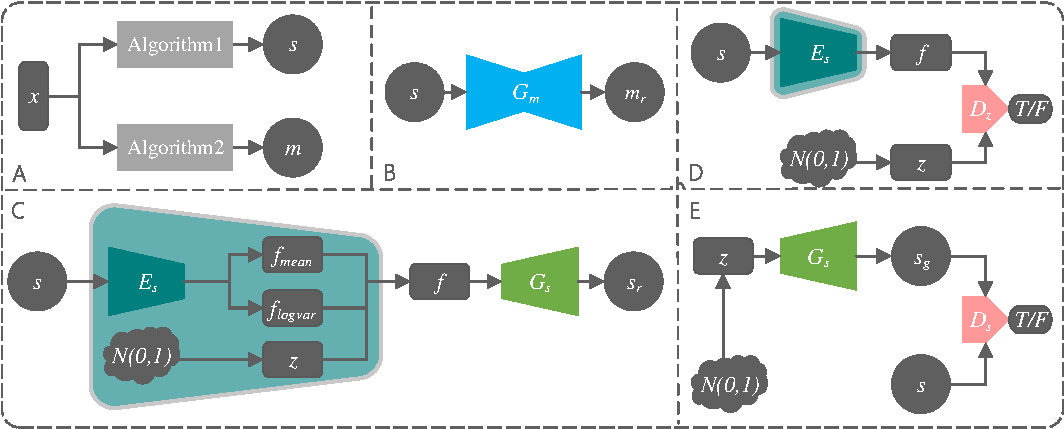
\includegraphics[width=1\columnwidth]{figures/feature_train}
		\caption{Structural map generation training. $x$ is an input real image, $s$ is a structural map, $m$ is a mask extract by Algorithm~\ref{alg:2}. $E_s$ is a VAE encoder, which outputs the encode matrixs $f_{mean}$ and $f_{logvar}$. $z$ is a random noise sampling from normal distribution $\mathcal{N}(0,1^2)$ and $f$ is a approximate normal distribution matrix. $G_s$ is a VAE decoder, $s_r$ is a reconstructed structural map, and $s_g$ is a synthesis structural map. $D_{s}$ and $D_{z}$ are the discriminators. $G_m$ is a mask generator and $m_r$ is a generated mask. $E_s $, $G_s$, $D_{z} $, $D_{s} $ are tuned on VGG11\cite{102simonyan2014very}, $G_m $ is tuned on U-net\cite{6zhu2017unpaired}. $E_s$ and all discriminators, including those described below, output two results in the last two layers. $G_s$ is a reverse VGG11. }
		\label{feature_train}
	\end{figure}
	The structural map generation training is shown in Fig.~\ref{feature_train}, where $f=f_{mean}+exp(0.5\times f_{logvar})\times z$. After training, the model can generate structural maps from random normal distribution matrixes. And Fig.~\ref{generated_f} shows examples of structural maps. The training losses in Fig.~\ref{feature_train} are as follows, where $\mathbb{E}$ is the expectation operator, and $m_r=G_m(s)$, $s_r=G_s(f)$, $s_g=G_s(z)$, $m_g=G_m(s_g)$: 
	\begin{itemize}
		\item{Part B: Mask generation loss}
		\begin{equation}
		\mathcal{L}_{m}(G_m)=\mathbb{E}_{m,s}[\Vert{m-m_r}\Vert_{2}^{2}],
		\end{equation}
		\item{Part C: Structural map reconstruction loss} 
		\begin{equation}
		\mathcal{L}_{r}(E_s,G_s)=\mathbb{E}_{s,f,m}[\Vert{s-s_r}\Vert_{2}^{2}+\Vert{m_r\times s_r}\Vert_{2}^{2}],
		\end{equation}
		\item{Part D: Distribution encoding adversarial loss} 
		\begin{equation}
		\mathcal{L}_{d1}(D_{z})=\mathbb{E}_{s,z}[\Vert{D_{z}(z)-1}\Vert_{2}^{2}+\Vert{D_{z}(f)}\Vert_{2}^{2}].
		\end{equation}
		\begin{equation}
		\mathcal{L}_{g1}(E_s)=\mathbb{E}_{z}[\Vert{D_{z}(f)-1}\Vert_{2}^{2}].	
		\end{equation}
		\item{Part E: Structural map decoding adversarial loss} 
		\begin{equation}
		\mathcal{L}_{d2}(D_{s})=\mathbb{E}_{s,z}[\Vert{D_{s}(s)-1}\Vert_{2}^{2}+\Vert{D_{s}(s_g)}\Vert_{2}^{2}].
		\end{equation}
		\begin{equation}
		\mathcal{L}_{g2}(G_s)=\mathbb{E}_{z}[\Vert{D_{s}(s_g)-1}\Vert_{2}^{2}++\Vert{m_g\times s_g}\Vert_{2}^{2}].	
		\end{equation}
	\end{itemize}
	\begin{figure}[th]
		\centering
		\includegraphics[width=1\linewidth]{figures/brats_f}
		\caption{Structural map on BRATS2015. (a) The images produced by structural map extraction. (b) Randomly-synthesized structural map. (c) Synthesized structural map from sequence sampling on normal distribution, where the output gradient effects is controlled by the gradient of the input. }
		\label{generated_f}
	\end{figure}
	\subsubsection{Fusion of Structural Map and Noise}	
	The structural map is a simple binary sparse matrix, which have less information and diversity. In general training, adding noise is one of the commonly uesd data enhancement method. Therefore, we define the equation $s'=s+z'\times(1-m)\times(1-s)$ to fuse random noise into the organ contour of the structural map, where $z'\sim\mathcal{U}(\alpha_1,\alpha_2)$, $\alpha_1 =0.5,\alpha_2=0.6$ by default. $m$ is a binary mask paired with the structual map $s$. As shown in Fig.~\ref{image_and_f}, the final fusion structural map $s'$ not only retains all the structure information, but also has rich random information. Moreover, it is closer to the expected medical image and thus easier to learn. 	
	\subsection{Multimodal Images Synthesis}
	As shown in Fig.~\ref{mm_mri_generate}, we use pre-trained $G_s$ to obtain $s_g$, then fuse with noise, the fusion can concatenate with the specified lesion label $l$. When selecting a lesion label randomly, the label may indicate a lesion that out of the organ contour in structural map. For this reason, we use the corresponding mask to filter out these labels that out of contour. Nextly, $G$ accepts the one-hot conditional matrix $one\_hot(i)$ and fusion input, and then decodes the input to generate the modality $i$ image $x_{g,i}$. The lesion processor $G_{l,i}$ and the modality translation network $G_t$ train completedly in advance to provide the lesions generation guidance loss and the registration guidance loss for $G$.
	\begin{figure}[th]
		\centering
		\includegraphics[width=1\linewidth]{figures/image_f_mask_newf}
		\caption{Medical image and the corresponding maps. (a) DRIVE retinal image. (b) Kaggle Chest Xray. (c) Kaggle Lung CT. (d) TC Lung CT.}
		\label{image_and_f}
	\end{figure}
	\begin{figure}[th]
		\centering
		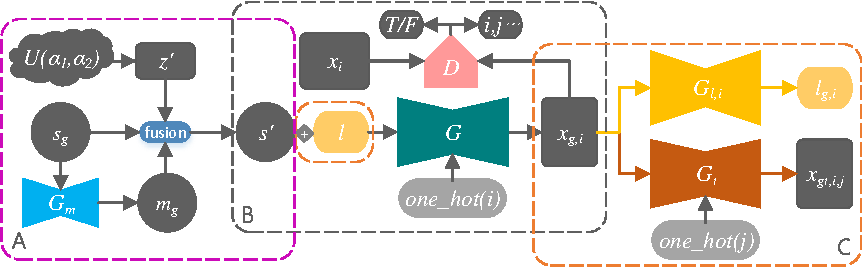
\includegraphics[width=1\columnwidth]{figures/mm_mri_generate_train}
		\caption{Synthesis of multimodal images. Purple box A is the fusion process of structural map and random noise, gray box B is the core synthesis process, and yellow box C is the optional refinement process. 
			$x_{g,i}$ is the image of modality $i$ generated by generator $G$. 
			$l_{g,i}$ is the lesion label of modality $i$ generated by lesion processor $G_{l,i}$.
			$x_{gt,i,j}$ is the image of modality $j$ translated from modality $i$ by modality translation network $G_t$.
		}
		\label{mm_mri_generate}
	\end{figure}
	
	$G$ and $D$ were tuned on U-net and VGG11 respectively and then formed a group of ACGAN\cite{98odena2016conditional} architecture. The loss items are as follows, where $d(x_{i})$ and $c(x_{i})$ are the true/false discrimination and category discrimination of the discriminator $D(x_i)$, $d(x_{g, i})$ and $c(x_{g,i})$ are the output of $D(x_{g,i})$, and $concat()$ is the concatenate operation on feture map channel. 
	\begin{itemize}
		\item{Adversarial loss}
		\begin{equation}
		\begin{split}
		\mathcal{L}_{d2}(D)=\mathbb{E}_{x,s_g,l}[\sum\limits_{i=0}(\Vert{d(x_i)-1}\Vert_{2}^{2}+\Vert{d(x_{g,i})}\Vert_{2}^{2}+\\
		\Vert{c(x_i)-i}\Vert_{2}^{2}+\Vert{c(x_{g,i})-i}\Vert_{2}^{2})],
		\end{split}
		\end{equation}
		\begin{equation}
		\mathcal{L}_{g}(G)=\mathbb{E}_{s_g,l}[\sum\limits_{i=0}(\Vert{d(x_{g,i})-1}\Vert_{2}^{2}+\Vert{c(x_{g,i})-i}\Vert_{2}^{2})].
		\end{equation}
		\item{Lesion generation guidance loss}
		\begin{equation}
		\mathcal{L}_{les}(G)=\mathbb{E}_{s_g,l}[\sum\limits_{i=0}(\Vert{l-l_{g,i}}\Vert_{2}^{2})].
		\end{equation}
		\item{Rregistration guidance loss}
		\begin{equation}
		\mathcal{L}_{reg}(G)=\mathbb{E}_{s_g,l}[\sum\limits_{j=0}\sum\limits_{i=0,i\neq j}(\Vert{x_{g,i}-x_{gt,j,i}}\Vert_{2}^{2})].
		\end{equation}
	\end{itemize}
	We can also use the real medical image and the structural map extracted from the real image for self-supervised pre-training to accelerate the process of adversarial training. The loss of the pre-training process is as follows:
	\begin{equation}
	\mathcal{L}_{p}(G)=\mathbb{E}_{s,l}[\sum\limits_{i=0}(\Vert{x_{g,i}-x_i}\Vert_{2}^{2}+\Vert{x_{g,i}\times m_i-x_{i}\times m_i}\Vert_{2}^{2})].
	\end{equation}
	In SkrGAN\cite{96zhang2019skrgan:}, real sketch training and self-supervision loss are always adopted, which result in over-fit on small datasets and lack of adaptability to synthesis sketch. This may eventually lead to the lack of diversity of synthesis image. We use real structure maps for self-supervised pre-training and use a large number of synthesis structure maps for adversarial training, which can not only accelerate the training process, but also enhance the generalization ability of model. Fig.~\ref{generated_mri} shows examples of images obtained from all stages on BRATS2015.
	\begin{figure}[th]
		\centering
		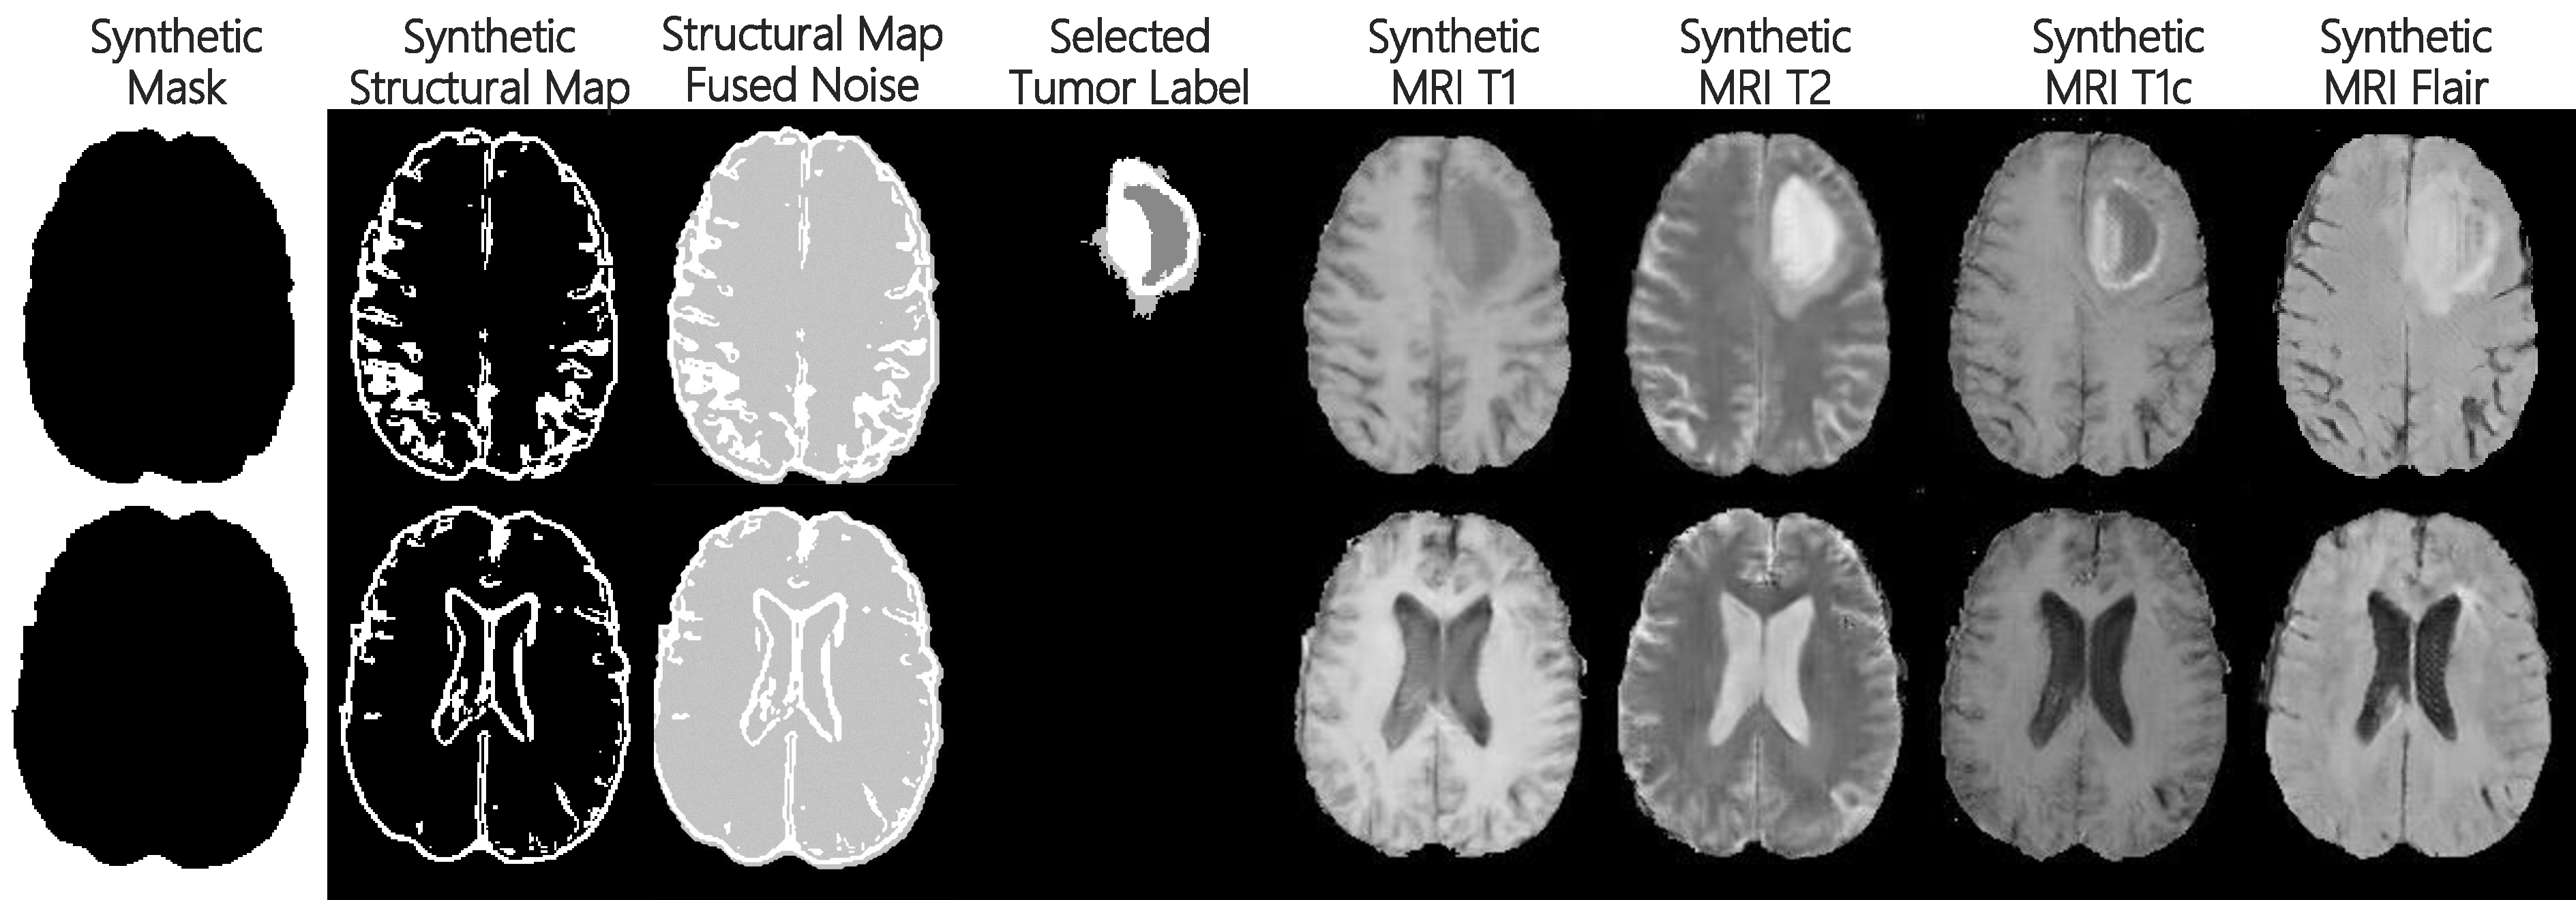
\includegraphics[width=0.8\linewidth]{figures/F_to_MRI}
		\caption{Multimodal images synthesis on BRATS2015.}
		\label{generated_mri}
	\end{figure}
	\subsection{Translation and Lesion Processing Training}
	Before multimodal images synthesis, we need to perform lesion processing and translation training on real data. $G_t$ and $D_t$ have the same structure and adversarial loss as $G$ together with $D$ and the cycle consistency loss in CycleGAN\cite{6zhu2017unpaired}.
	U-net and SSD\cite{101liu2016ssd:} were used for segmentation and detection as the lesion processor $G_l$. The loss of $G_{l,i}$ is same as in multimodal images synthesis stage, except that the real labels $l_i$ are used.
	\section{Experiments}
	\subsection{Datasets}
	\textbf{BRATS2015\footnote{https://www.smir.ch/BRATS/Start2015}} includes registered T1, T2, T1c, Flair, 274 [155$\times$240$\times$240] MRIs per modality, and the correspoding tumor segmentation labels. \textbf{Kaggle Chest Xray\footnote{https://www.kaggle.com/paultimothymooney/chest-xray-pneumonia }} includes 5863 positive Xray from size [384$\times$127] to [2772$\times$2304]. \textbf{Kaggle Lung CT\footnote{https://www.kaggle.com/kmader/finding-lungs-in-ct-data/data/}} includes 267 CT of transverse from lung, with a size of [512$\times$512]. \textbf{DRIVE\footnote{http://www.isi.uu.nl/Research/Databases/DRIVE/}} includes 20 [565$\times $584] color fundus retinal photos and corresponding retinal vascular segmentation annotations in both training set and test set. \textbf{FIRE\footnote{https://projects.ics.forth.gr/cvrl/fire/}} includes 268 [2912$\times$2912] color fundus retinal photos. 
	\textbf{TC Lung CT\footnote{https://tianchi.aliyun.com/competition/entrance/231724/information}} includes 1470 [512$\times$512] 3D CT with detection label of 5 kinds of lesions. We only examined for pulmonary nodules. We divided all 3D images to 2D sildes. All images are normalized and scaled to [512$\times$512].
	\begin{table}[th]
		\newcommand{\tabincell}[2]{\begin{tabular}{@{}#1@{}}#2\end{tabular}}
		\caption{Ablation experiments on BRATS2015}
		\label{Ablation Experiment Setting on BRATS2015}
		\centering
		\resizebox{0.8\textwidth}{12.5mm}{
			\begin{tabular}{c|c|c|c|c|c|l}
				\hline
				Test		&\tabincell{c}{Noise} &\tabincell{c}{Structural map} &\tabincell{c}{$\mathcal{L}_{reg}$} &\tabincell{c}{Lesion label, $\mathcal{L}_{les}$} &\tabincell{c}{Filter lesion label} &MS-SSIM \\
				\hline
				\tabincell{l}{A}	&$\surd$	&$\times$	&$\times$	&$\times$	&$\times$ &0.504 \\
				\tabincell{l}{B}	&$\times$	&$\surd$	&$\times$	&$\times$ &$\times$ &0.654\\
				\tabincell{l}{C}	&$\surd$	&$\surd$	&$\times$	&$\times$	&$\times$ &0.671\\
				\tabincell{l}{D}	&$\surd$	&$\surd$	&$\surd$	&$\times$	&$\times$ &0.674\\
				\tabincell{l}{E}	&$\surd$	&$\surd$	&$\surd$	&$\surd$	&$\times$ &0.673\\
				\tabincell{l}{F}	&$\surd$	&$\surd$	&$\surd$	&$\surd$	&$\surd$ &\textbf{0.686}\\
				\hline
			\end{tabular}
		}
	\end{table}
	\begin{figure}[th]
		\centering
		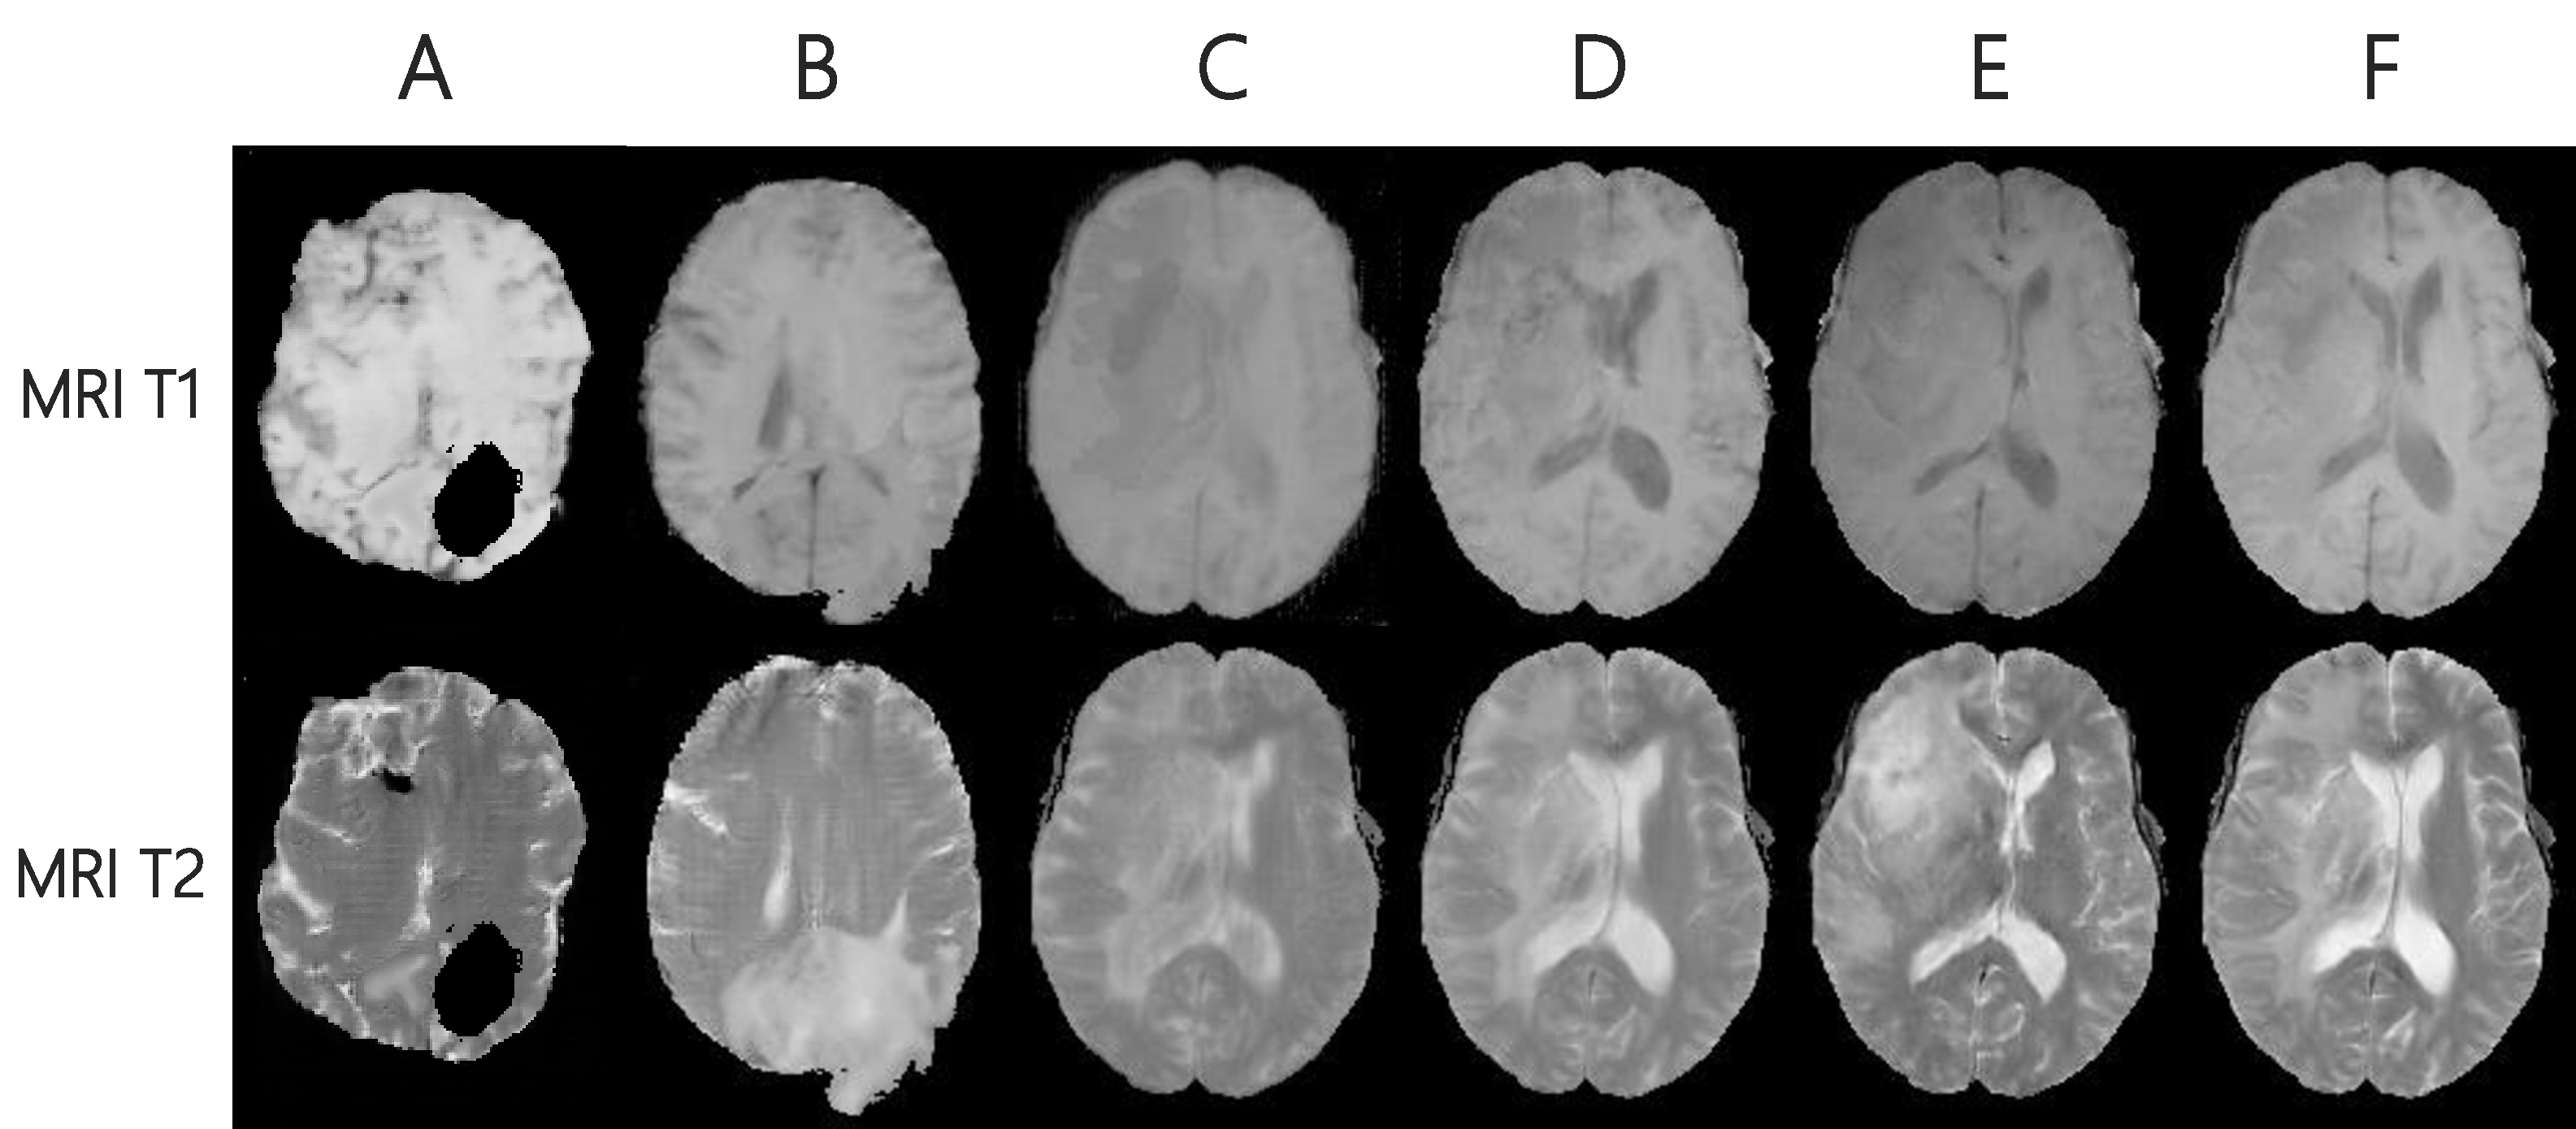
\includegraphics[width=0.9\linewidth]{figures/ablation}
		\caption{(a) Synthetic MRIs of ablation experiments. (b) Segmentation results of synthetic MRI. }
		\label{ablation_and_seg}
	\end{figure}
	\begin{table}[th]
		\begin{center}
			\caption{Lesion generation methods experiments.}
			\label{label_test}
			\resizebox{0.48\textwidth}{6mm}{
				\begin{tabular}{llccc}
					\hline	
					Trainging Dataset &Test Dataset &MSE &Dice score \\
					\hline
						real &real 	 &0.027   &0.915 \\							
						real &synthetic	&0.098 &0.838 \\
					\hline
			\end{tabular}}
		\end{center}
	\end{table}
	\subsection{Experiments Settings}
	Each experiment is comprehensively trained with more than 100 epochs with the environment of Python3.6+TensorFlow1.13 on NVIDIA Tesla V100GPU cluster. The learning rate is 1e-5 with 4 batch size. We use the Adam optimizer with beta1 of 0.5.
	The state-of-the-art synthesis method SkrGAN\cite{96zhang2019skrgan:} is our benchmark. We used multi-scale structural similarity (MS-SSIM) and FreshetInception distance (FID)\cite{100karras2017progressive} to assess the performance of synthetic medical images. Dice Score\cite {95dice1945measures} and mean square error (MSE) are used to evaluate the segmentation results. Sensitivity, Accuracy and area under the ROC curve (AUC) are used to assess vascular annotation results. The Average Precision (AP) is used to estimate the detection results. We evaluate on 2D and adpot the best results after at least four training sessions.	
	\subsection{Ablation Experiments on BRATS2015}
	Table~\ref{Ablation Experiment Setting on BRATS2015} shows the settings and results of the ablation experiments of our method.
	Fig.~\ref{ablation_and_seg} (a) shows examples of synthetic images generated in ablation experiments. 
	\textbf{A} no contour from structural map, the synthetic image conforms to the features of MRI, but not to the structural features of the brain. 
	\textbf{B} was poorly trained due to lack of a random sample.
	\textbf{C} registration effect seems unsatisfactory, especially the edge details.
	Lesions in \textbf{D} are random and exaggerated, which hardly match the input label. 
	Obviously, tumor in \textbf{E} is beyond the contours of the brain. 
	\textbf{F} adopts our complete scheme and achieve best synthesis quality. The results show that our method is helpful to improve the authenticity of the synthesized image. However, the lesion labels need to be screened before input.
	
	\subsection{Evaluation of Lesion Effectiveness on BRATS2015}
	\label{label gen methods tests}
	As shown in Table~\ref{label_test} and Fig.~\ref{ablation_and_seg} (b), the segmentation model trained with real data can be used for the synthetic data, indicating that the distribution synthetic data are very similar to that of real data, and the synthetic lesions and the real lesions are similar enough for the segmentation model to recognize the synthetic lesions and non-focal parts. The results show that synthetic lesions are effective.
	\begin{table}[th]
		\newcommand{\tabincell}[2]{\begin{tabular}{@{}#1@{}}#2\end{tabular}}
		\begin{center}
			\caption{Evaluation of synthetic images quality (A)}
			\label{evalu_on_all_dataset1}
			\resizebox{\textwidth}{9.7mm}{
				\begin{tabular}{ll|llllll}
					\hline
					Dataset &Metric &Ours &SkrGAN\cite{96zhang2019skrgan:} &DCGAN\cite{97radford2015unsupervised,96zhang2019skrgan:} &ACGAN\cite{98odena2016conditional,96zhang2019skrgan:} &WGAN\cite{99arjovsky2017wasserstein,96zhang2019skrgan:} &PGGAN\cite{100karras2017progressive,96zhang2019skrgan:}\\
					\hline
					\multirow{2}*{\tabincell{l}{\textbf{Kaggle}\\\textbf{Chest Xray}}}
					&MS-SSIM $\uparrow$ &\textbf{0.597} &0.506 &0.269 &0.301 &0.401 &0.493 \\
					&FID $\downarrow$ &\textbf{102.5} &114.6 &260.3 &235.2 &300.7 &124.2\\
					\hline
					\multirow{2}*{\tabincell{l}{\textbf{Kaggle}\\\textbf{Lung CT}}}
					&MS-SSIM $\uparrow$ &\textbf{0.473} &0.359 &0.199 &0.235 &0.277 &0.328 \\
					&FID $\downarrow$ &\textbf{66.91} &79.97 &285.0 &222.5 &349.1 &91.89\\
					\hline
			\end{tabular}}
		\end{center}
	\end{table}
	\subsection{Evaluation of Synthetic Images Quality }
	As shown in Table~\ref{evalu_on_all_dataset1}-~\ref{evalu_on_all_dataset2}, our method is quantitatively evaluated on various datasets and compared with the state-of-the-art methods. Combined the results in tables with the visual comparison in Fig.~\ref{evalu_compare}, the quality of the synthetic image input with structural map is much better than that of the synthetic image input with random noise. The model generalizes better when the structural map is processed by fusion noise versus those processe without fusion noise or treated by binary inversion. Self-supervised pre-training can improve the quality of synthetic image obviously. Compared with the sketch of SkrGAN and other random noise input, the structural map, self-supervised pre-training, lesion loss and other measures that we adopted make the synthetic medical image in this study achieve higher quality and closer to the real image.
	\begin{table}[th]
		\newcommand{\tabincell}[2]{\begin{tabular}{@{}#1@{}}#2\end{tabular}}
		\begin{center}
			\caption{Evaluation of synthetic images quality (B)}
			\label{evalu_on_all_dataset2}
			\resizebox{0.6\textwidth}{11.5mm}{
				\begin{tabular}{ll|llll}
					\hline
					Dataset &Metric &Our tumor &Ours &SkrGAN$^*$ &Basic GAN\\
					\hline
					\multirow{2}*{\tabincell{l}{\textbf{DRIVE+FIRE}\\\textbf{Color Fundus}}}
					&MS-SSIM $\uparrow$ &-  &\textbf{0.607} &0.584 &0.392\\
					&FID $\downarrow$  &-  &\textbf{30.13} &37.91 &227.41\\
					\hline
					\multirow{2}*{\tabincell{l}{\textbf{BRATS2015}\\\textbf{MRI}}}
					&MS-SSIM $\uparrow$ &0.692 &\textbf{0.686} &0.653 &0.504\\
					&FID $\downarrow$  &20.15 &\textbf{21.87} &28.76 &124.53\\
					\hline
					\multirow{2}*{\tabincell{l}{\textbf{TC Lung }\textbf{CT}}}
					&MS-SSIM $\uparrow$ &-  &\textbf{0.676} &0.667 &0.543\\
					&FID $\downarrow$  &-  &\textbf{27.40} &29.81 &113.65\\
					\hline
			\end{tabular}}
			\footnotesize
			\item[*] The reproduce SkrGAN trains on the inverse binary image of our real structure map.
		\end{center}
	\end{table}
	\begin{table}[th]
		\begin{center}
			{\caption{Synthetic data availability verification on BRATS2015 tumor segmentor.}\label{availability_test}}
			\resizebox{0.5\textwidth}{25mm}{
				\begin{tabular}{llllcc}
					\hline
					Real &Synthetic & Enhanced & Mix & MSE &Dice score\\
					\hline		
					 $\times$1      & 0 			&0 			&- 				&0.027 &0.915 \\
%					 $\times$50\%   & 0  			&0 			&- 				&0.041 &0.900 \\
					 0 	 	        & $\times$1 	&0 			&- 				&0.294 &0.708 \\	
%					 0 	 	        & $\times$2  	&0 			&- 				&0.253 &0.736 \\
%					 0 		        & $\times$3  	&0 			&-				&0.251 &0.738 \\
					 $\times$10\% 	& $\times$1  	&0 			&$\mathcal{S}$ &0.036 &0.906 \\
%					 $\times$10\% 	& $\times$2     &0 			&synthetic first&0.034 &0.907 \\
%					 $\times$10\% 	& $\times$3     &0 			&synthetic first&0.033 &0.907 \\
					 $\times$20\% 	& $\times$80\% 	&0 			&$\mathcal{M}$ 	&0.038 &0.904 \\
%					 $\times$50\% 	& $\times$50\% 	&0  		&random mixing  &0.031 &0.909 \\
					 $\times$80\% 	& $\times$20\% 	&0 			&$\mathcal{M}$ 	&0.028 &0.914 \\
					 $\times$1 	 	& $\times$20\%  &0 			&$\mathcal{M}$ 	&0.025 &0.921 \\
					 $\times$1 	 	& $\times$50\%  &0 			&$\mathcal{M}$ 	&\textbf{0.020} &\textbf{0.939} \\
%					 $\times$1 	 	& $\times$80\%	&0  		&random mixing  &0.021 &0.937 \\
					 $\times$1 	 	& $\times$1		&0 			&$\mathcal{M}$ 	&0.022 &0.934 \\
%					 $\times$1 	 	& $\times$2   	&0 			&random mixing  &0.023 &0.931 \\
%					 $\times$1 	 	& $\times$3   	&0 			&random mixing  &0.023 &0.930 \\
					 $\times$1 	 	&0 				&$\times$20\%&$\mathcal{M}$ &0.027 &0.917 \\
					 $\times$1 	 	&0 				&$\times$50\%&$\mathcal{M}$ &0.025 &0.920 \\
%					 $\times$1    	&0 				&$\times$80\%&random mixing &0.026 &0.920 \\
					 $\times$1 	 	&0 				&$\times$1 &$\mathcal{M}$ 	&0.026 &0.919 \\
%					 $\times$1 	 	&0 				&$\times$2  &random mixing 	&0.026 &0.919 \\
%					 $\times$1 	 	&0 				&$\times$3  &random mixing 	&0.027 &0.918 \\	
					 $\times$1 	 	& $\times$1 	&0 			&$\mathcal{R}$ 	&0.161 &0.795 \\
					 $\times$1 	 	& $\times$1 	&0 			&$\mathcal{S}$ 	&\textbf{0.020} &\textbf{0.940}
					\\
					\hline
					\multicolumn{6}{l}{$\mathcal{M}$: random mixing\ \
						$\mathcal{S}$: synthetic first\ \
						$\mathcal{R}$: real first}
			\end{tabular}}
		\end{center}
	\end{table}
	\begin{table}[th]
		\newcommand{\tabincell}[2]{\begin{tabular}{@{}#1@{}}#2\end{tabular}}
		\begin{center}
			\caption{Synthetic data availability verification on DRIVE vascular segmentor.}
			\label{DRIVE_availability_test}
			\resizebox{0.8\textwidth}{9.5mm}{
				\begin{tabular}{clccc}
					\hline
					Training Data &Test Data &Sensitivity &Accuracy &AUC\\
					\hline
					\tabincell{c}{Training Set} 	 	& Test Set 	&0.7781 &0.9477 &0.9705
					\\
					\tabincell{c}{Training Set+2000 SkrGAN Synthetic Images}	 & Test Set 	& \textbf{0.8464} &0.9513 &\textbf{0.9762} \\
					\tabincell{c}{Training Set+2000 SkrGAN$^*$ Synthetic Images}	 & Test Set 	& 0.8297 &0.9428 &0.9732 \\
					\tabincell{c}{Training Set+2000 Our Synthetic Images}	& Test Set 	&0.8416&\textbf{0.9518 }&0.9749 \\	
					\hline
			\end{tabular}}
			\footnotesize
			\item[*] The reproduce SkrGAN trains on the inverse binary image of our real structure map.
		\end{center}
	\end{table}
	\begin{table}[th]
		\newcommand{\tabincell}[2]{\begin{tabular}{@{}#1@{}}#2\end{tabular}}
		\begin{center}
			\caption{Synthetic data availability verification on TC Lung CT pulmonary nodule detector.}
			\label{TC_availability_test}
			\resizebox{0.8\textwidth}{6mm}{
				\begin{tabular}{clllc}
					\hline
					Training Data &Test Data & AP \\
					\hline
					\tabincell{c}{TC Lung CT Training Set} 	 	&\tabincell{c}{TC Lung CT Test Set} 	&0.574 
					\\
					\tabincell{c}{TC Lung CT Training Set + 20000 Synthetic Images}	&\tabincell{c}{TC Lung CT Test Set} 	&\textbf{0.592} \\	
					\hline
			\end{tabular}}
		\end{center}
	\end{table}
	\subsection{Evaluation of Synthetic Data Availability}
	As shown in Table~\ref{availability_test}, we mixed real BRATS2015 training data with synthetic data in different amounts, then we used the mixed data for segmentation training, and finally evaluated the segmentation ability of the model on the real BRATS2015 test dataset. We set up three data mixing modes: random mixing, real data training first, and synthetic data training first. As reported in Table~\ref{availability_test}, our synthetic images can be used as pre-trained data or enhanced data to greatly improve the generalization ability of the model, and the performance of our synthetic data augmentation is much better than the usual data augmentation. We do not recommend using synthetic data completely for training or using synthetic data for supplementary training.
	
	Similarly in Table~\ref{DRIVE_availability_test}-\ref{TC_availability_test}, we performed other medical image processing tasks with the medical images synthesized on other datasets. The results show that our synthetic data can also improve the generalization ability of the model in these tasks, which indicates that our synthetic data are available and the synthetic lesions are effective.
	\begin{figure}[th]
		\centering
		\includegraphics[width=0.78\linewidth]{figures/evalu_compare}
		\caption{Visual contrast of synthetic images. In SkrGAN lines are synthetic image of SkrGAN\cite{96zhang2019skrgan:}, the input sketch and the sketch binary inversion image. In Our lines are our synthetic image, the input structural map fusioned noise and the original structural map.}
		\label{evalu_compare}
	\end{figure}
	\section{Conclustion}
	In this paper, a clearer extraction method of medical image structural map based Sobel operator is proposed, which requires no training or additional labels, and takes advantage of VAE to learn the mapping between normal distribution and structure map distribution. The multimodal synthesis based on structural maps can synthesize the medical image that conforms to physiological structure. The well designed lesion generation guidance loss and registration supervision loss ensure the synthesis of the specified lesion and multimodal registration. Experimental results on multiple datasets show that the synthetic lesions are effective, and the synthetic medical images can be used as pre-trained data or enhanced data to improve the performance of the model.
	%
	% ---- Bibliography ----
	%
	% BibTeX users should specify bibliography style 'splncs04'.
	% References will then be sorted and formatted in the correct style.
	%
	\bibliographystyle{splncs04}
	\bibliography{mybibliography}	
\end{document}